\documentclass[12pt,a4paper]{article}
\usepackage[utf8]{inputenc}
\usepackage{xeCJK}
\usepackage{amsmath}
\usepackage{amsthm}
\usepackage{mathtools}
\usepackage{amsfonts}
\usepackage{amssymb}
\usepackage{graphicx}
\usepackage{epigraph}
\usepackage[left=2cm,right=2cm,top=2cm,bottom=2cm]{geometry}
\usepackage{etoolbox}
\usepackage{fancyhdr}
\usepackage{hyperref}

\newtheorem{theorem}{Theorem}
\newtheorem{lemma}{Lemma}
\graphicspath{ {/Users/zhangyutong926/Workspace/GeneralWork/EXModeling/shortest_path/} }

\pagestyle{fancy}
%%
\lhead{$\text{星宮}\,\text{清子}$、$\text{雨宮}\,\text{祐子}$}
\rhead{Calculi Variationum Microdiastimeque}
%%
\renewcommand{\headrulewidth}{0.4pt}

\newtheorem{definition}{Definition}
\newtheorem{assertion}{Assertion}
\DeclarePairedDelimiter\abs{\lvert}{\rvert}
\setlength{\parindent}{0em}
\setlength{\parskip}{.5em}
\epigraphsize{\small\itshape}
\setlength\epigraphwidth{12cm}
\setlength\epigraphrule{0pt}
\setCJKmainfont{ipaexm.ttf}
\newcommand\bibname{References}

\makeatletter
\patchcmd{\epigraph}{\@epitext{#1}}{\itshape\@epitext{#1}}{}{}
\makeatother
\newcommand{\MRef}[2]{\hyperref[#2]{#1 \ref*{#2}}}
\newcommand{\eqnref}[1]{(\ref{#1})}

\author{$\text{星宮}\,\text{清子}$\\(Hoshi-no-miya Sayako)\and$\text{雨宮}\,\text{祐子}$\\(Ame-no-miya Sachiko)}
\date{}
\title{Calculi Variationum Microdiastimeque}

\begin{document}
\maketitle
\epigraphsize{\small\itshape}
\epigraph{``The shortest path between two points is a straight line."}{--- \textup{Menelaus of Alexandria}, Sphaerica \textup{\cite{meneclaus}}}
%\begin{abstract}
%In this article we will explore the measure of length in Euclidean spaces by Riemann Sum and Riemann Integral and the property of the extremae of functionals $\left(\mathbb{R}\to\mathbb{R}\right)\to\mathbb{R}$ \cite{euler_calc_var} and then $\left(\mathbb{R}\to\mathbb{R}\right)^n\to\mathbb{R}$ \cite{weinstock_calc_var}, which would establish a foundation for a proof of a fundamental property in $\mathbb{R}^k$ --- the shortest path between two points is a straight line, also we will explore the brachistochrone curve as an application of calculus of variation.
%\end{abstract}

\section{Introduction}
We will start our investigation with a classical but non-trivial problem, and we will come back to it at the end of the article to conclude it.

\begin{theorem}[Meneclaus \cite{meneclaus}]
\label{thm:microdiastime}
The shortest path between two points in $\mathbb{R}^k$ is a straight line.
\end{theorem}

The statement of the theorem itself dates back to the age of Meneclaus and Euclid, but now with modern mathematics in mind we must restrict our discussion strictly in Euclidean space, i.e. $\mathbb{R}^k$, since it is facile to construct counter-examples outside Euclidean spaces. As our discussion progresses, we will generalize our concepts of straight lines, but for now we will only consider a direct-proportion function in $\mathbb{R}^2$ as a line.

As we shall see, the methodology we developed in this article is a part of a broader theory --- analytical mechanics, to be more specific, Lagrangian mechanics --- which is a modern branch of theoretical mechanics that specifically refines the Newtonian mechanics in handling complicated mechanical constraints. The application of this methodology will be revealed, in the second part of the article, by several examples including the Brachistochrone problem, the mathematical model of the motion in Sphyrobolie, and the mathematical model of a generic double pendula.

\section{Measure of Length}
There are many way one can define length of curve as, the most famous and predominant among which would be the Lebesgue outer measure \cite{lebesgue_outer_measure}
\[
\Lambda(E) = \operatorname{inf} \left\{\sum_{k=1}^\infty \ell(I_k) : {(I_k)_{k \in \mathbb N}} \text{ is a finite collection of open intervals with } E\subseteq \bigcup_{k=1}^\infty I_k\right\}
\]
where $E\subseteq\mathbb{R}$, with the length of interval $I = (a, b)$ given by $\ell(I)= b - a$, but in this article an alternative measure --- using Riemann integral \cite{riemann_sum_integral} --- for length in $\mathbb{R}^k$ is defined.

The discussion of length measure in $\mathbb{R}^k$ begins from its simplest special case: a function-defined curve in $\mathbb{R}^2$, and then shifts to the generic curves defined by parametric equations in $\mathbb{R}^k$.

\subsection{Function-Defined Curve in $\mathbb{R}^2$}
For a curve defined by function $f(x)$ on $\mathbb{R}^2$, to calculate the length from point $(a,f(a))$ to $(b,f(b))$, we partition the interval $[a,b]$ into n parts, with $x_0,x_1,x_2,\dots,x_n$ denoting their corresponding boundary. Now if one denotes the points on curve \[P_i:=(x_i,f(x_1))\quad\text{where }i=0,1,2,\dots,n,\] there would be an approximation \begin{gather}\label{eqn:length_approx}L\approx\sum_{i=1}^n\abs{\overline{P_{i-1}P_i}}=\sum_{i=1}^n\sqrt{(x_i-x_{i-1})^2+(y_i-y_{i-1})^2}.\end{gather} One example when $n=10$ of $f(x)=\sin x$ is shown in Figure \ref{fig:differential_element_length}.

\begin{figure}[htbp]
    \centering
    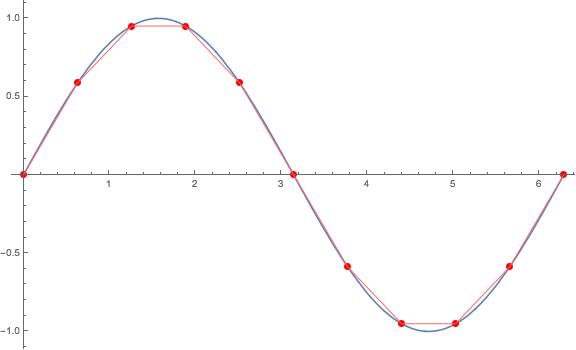
\includegraphics[scale=0.7]{differential_element_length.png}
    \caption{Demonstration of differential elements method in calculating length}
    \label{fig:differential_element_length}
\end{figure}

With Newton's principle of differential elements \cite{newton_pnpm} and \eqnref{eqn:length_approx}, the exact value of length would be \begin{gather}\label{eqn:riemann_sum_unsimpl}L=\lim_{n\to+\infty}\sum_{i=1}^n\sqrt{(x_i-x_{i-1})^2+(y_i-y_{i-1})^2}.\end{gather} Note that the partition density increases during the limit process. The form of the expression of length becomes a Riemann sum \cite{riemann_sum_integral}, but before it is rewritten in Riemann integral \cite{riemann_sum_integral}, its form is to be simplified by expressing \eqnref{eqn:riemann_sum_unsimpl} as \begin{gather}\label{eqn:length_with_delta}L=\lim_{n\to+\infty}\sum_{i=1}^n\sqrt{\Delta x_i^2+\Delta y_i^2}\end{gather} where $\Delta x_i=x_i-x_{i-1},\, \Delta y_i=y_i-y_{i-1}$.

With Lagrange's Mean-Value Theorem (Corollary to Rolle's Theorem \cite{drobisch_rolle_theorem}), it is always possible to find $\xi_i\in[x_{i-1},x_i]$ such that \[f'(\xi_i)=\frac{y_i-y_{i-1}}{x_i-x_{i-1}}=\frac{\Delta y_i}{\Delta x_i},\] and write \begin{gather}\label{eqn:length_with_xi}L=\lim_{n\to+\infty}\sum_{i=1}^n\sqrt{\Delta x_i^2+\Delta x_i^2f'(\xi_i)^2}=\lim_{n\to+\infty}\sum_{i=1}^n\sqrt{1+f'(x_i)^2}\cdot\Delta x_i,\end{gather} since $\xi_i\to x_i$ when $n\to0$ (assuming the partition is done uniformly).

Now it is appropriate to use the integral notation for rewriting \eqnref{eqn:length_with_xi}, since the expression has matched the definition of Riemann integral \cite{riemann_sum_integral}.

\begin{definition}[Length of Function-Defined Curve in $\mathbb{R}^2$]\label{def:length_func_bi}
Given a function $f:\mathbb{R}\to\mathbb{R}$ with continuous derivative, the length of the curve defined by the function in interval $[a,b]$ is defined as
\begin{gather}
\label{eqn:length_func}
\int_a^b\sqrt{1+f'(x)^2}\,\mathrm{d}x.
\end{gather}
\end{definition}

\subsection{Parametric Curve in $\mathbb{R}^k$}
In the previous subsection the length measure of a function-defined curve in $\mathbb{R}^2$ is investigated, and now a generalization is expected.

\begin{definition}[Parametric Curve in $\mathbb{R}^k$]
A system of parametric equations
\[
\begin{dcases}
x_1=f_1(t)\\
x_2=f_2(t)\\
\vdots\\
x_k=f_k(t)
\end{dcases}
\]
is said to be a curve in n-dimensional Euclidean space $\mathbb{R}^k$.
\end{definition}

Apply the similar technique and define the length measure for parametric curves in $\mathbb{R}^k$. With a given $n$, assume interval $[a,b]$ is partitioned into n parts where $t_0=a,\,t_n=b,$ and the rest of $t_i$ being the boundaries of parts, then with $P_i=(x_1(t_i),\,x_2(t_i),\dots,\,x_n(t_i))$, the length would be
\begin{align}
L&=\lim_{n\to\infty}\sum_{i=1}^n\,\abs{\overline{P_i\,P_{i-1}}}\\
\label{eqn:para_length_no_delta}&=\lim_{n\to\infty}\sum_{i=1}^n\sqrt{\sum_{j=1}^k\left(x_j(t_i)-x_j(t_{i-1})\right)^2}.
\end{align}

Employ the same notation for offsets in independent variable $t$ and each of the components of the parametric equations
\[
\begin{dcases}
\Delta t_i=t_i-t_{i-1}\\
\Delta x_{1,i}=x_1(t_i)-x_1(t_{i-1})\\
\Delta x_{2,i}=x_2(t_i)-x_2(t_{i-1})\\
\vdots\\
\Delta x_{k,i}=x_k(t_i)-x_k(t_{i-1})
\end{dcases}.
\]

\eqnref{eqn:para_length_no_delta} can be rewritten as
\begin{gather}
\label{eqn:para_length_delta}
L=\lim_{n\to\infty}\sum_{i=1}^n\sqrt{\sum_{j=1}^k{\Delta x_{j,i}}^2}.
\end{gather}

Once again continuously apply Lagrange Mean Value Theorem \cite{drobisch_rolle_theorem} for $k$ times, obtaining $\xi_{1,i},\,\xi_{2,i},\dots,\,\xi_{k,i}$ such that
\[
{f_j}'(\xi_{j,i})=\frac{x_j(t_i)-x_j(t_{i-1})}{t_i-t_{i-1}}\,\text{ for all } j=1,2,\dots,k,
\]
and rewriting \eqnref{eqn:para_length_delta} as
\begin{align}
L&=\lim_{n\to\infty}\sum_{i=1}^n\sqrt{\sum_{j=1}^k{\Delta t_i}^2{x_j}'(\xi_{j,i})^2}\\
\label{eqn:para_length_riemann_sum}&=\lim_{n\to\infty}\sum_{i=1}^n\left(\sqrt{\sum_{j=1}^k{x_j}'(t_i)^2}\cdot{\Delta t_i}\right),
\end{align}
since $\xi_{j,i}\to t_i$ for $j=1,2,\dots,k$ when $n\to\infty$.

Once again \eqnref{eqn:para_length_riemann_sum} identifies with Riemann sum, which produces an equivalent notation to Riemann integral.
\begin{definition}[Length of Parametric Curve in $\mathbb{R}^k$]\label{def:length_para}
Given a system of $k$ parametric equations defining a curve in $\mathbb{R}^k$, each of which has a continuous derivative, the length of the curve from the point where $t=a$ to where $t=b$ is defined as
\begin{gather}
\label{eqn:length_para}
\int_a^b\left(\sum_{j=1}^k{x_j}'(t)^2\right)^{\frac{1}{2}}\mathrm{d}t.
\end{gather}
\end{definition}

\section{Stationary Functions of Functional}
From Definition \ref{def:length_func_bi} and \ref{def:length_para}, we instinctively consider a generalization of the notion of function: $L[f]:(\mathbb{R}\to\mathbb{R})\to\mathbb{R}$ and $L[x_1,\,x_2,\dots,\,x_k]:(\mathbb{R}\to\mathbb{R})^k\to\mathbb{R}$, which are called functionals in modern mathematics by, presumably, Leonhard Euler \cite{euler_calc_var}. To be more specific, the goal of this section is to investigate the analogy of functions' stationary points in the context of functionals, the stationary functions, and, obviously, their property. We will be able to conclude, at the end of this section, a sufficient and necessary condition for a function to be a stationary function of a functional, and, not surprisingly, the same condition as the necessary condition of a function being a functional's minimum or maximum, for two specific kind of functional, the Euler-Lagrange equation \cite{euler_calc_var} \cite{weinstock_calc_var}, and a generalized version for multiple functions. Unfortunately, the second-order partial derivative of a multi-variable functional does not have an equally elegant representation, and thus the discussion of if would be omitted from this article.

\subsection{Extremization Condition for Functional of Single Uni-Variable Function with First-Order Derivative}
\begin{lemma}[Fundamental Lemma of Calculus of Variations]
\label{lem:fundamental}
If
\[
\int_a^b f(x)\,\eta(x)\,\mathrm{d}x = 0\quad\forall\eta(x),
\]
then
\[
f(x)=0\quad\forall x\in[a,b]
\]
where $f(x)$ and $\eta(x)$ is continuously differentiable over $[a,b]$ and $\eta(a)=\eta(b)=0$.\footnote{Some text uses the condition that $\eta(x)$ is compactly supported on $[a,b]$.}
\end{lemma}
\begin{proof}
The proof is trivial by contradition. Assume, without loss of generality, $\exists x_0\in[a,b].\,f(x)>0$, then $\exists (m,n)\in[a,b].\,\forall x\in(m,n).\,f(x)>0$ since $f(x)$ is continuous. By the assumption of $f(x)$ and Weierstrass Extreme Value Theorem \cite{rudin_principles}, there is a $u>0$ such that $\displaystyle u=\min_{x\in[a,b]}f(x)$. Fixing an arbitrarily large $M$, define $\displaystyle \eta(x)=\frac{M}{u}$, then the value of the integral would be $M$, which contradicts the assumption that the value of the integral is $0$, quod erat demonstradum.
\end{proof}

\begin{theorem}[Euler-Lagrange \cite{euler_calc_var}]
\label{thm:euler_lagrange}
For a given functional
\begin{gather}
\label{eqn:euler_lagrange_functional}
I[f]=\int_a^bF(x,f(x),f'(x))\,\mathrm{d}x
\end{gather}
where
\begin{align*}
f:[a,b]\subset\mathbb{R}&\to\mathbb{R}\\
x&\mapsto f(x)\\
f(a)&=A\\
f(b)&=B,
\end{align*}
and
\begin{align*}
F:[a,b]\times\mathbb{R}^2&\to\mathbb{R}\\
(x,f(x),f'(x))&\mapsto F(x,f(x),f'(x)),
\end{align*}
\footnote{Note that the original formulation of the condition \cite{euler_calc_var} is written in the language of differential geometry, tangent spaces and tangent bundles to be more specific, and for the simplicity of this article we have omitted the concepts from differential geometry and focus our discussion only on the real numbers instead of any arbitrary vector space; and also that in \cite{euler_calc_var} and \cite{weinstock_calc_var}, the equation is written in the form of \eqnref{eqn:euler_lagrange} instead of \eqnref{eqn:euler_lagrange_tedious}, for the omitted parts is semantically insignificant due to their triviality.}
where $F$ is continuously differentiable up to second-order with respect to all parameters, then the condition of a function $f_0(x)$ being a stationary function, or the necessary but not sufficient condition of the same function being the maximum or minimum function is that
\begin{gather}
\label{eqn:euler_lagrange_tedious}
\frac{\partial}{\partial f_0(x)}F(x,f_0(x),{f_0}'(x))-\frac{{\mathrm{d}}}{\mathrm{d}x}\left(\frac{\partial}{\partial {f_0}'(x)}F(x,f_0(x),{f_0}'(x))\right)=0,
\end{gather}
or in a more concise and implicit expression,
\begin{gather}
\label{eqn:euler_lagrange}
\frac{\partial}{\partial f_0}F-\frac{\mathrm{d}}{\mathrm{d}x}\left(\frac{\partial}{\partial {f_0}'}F\right)=0.
\end{gather}
\end{theorem}
\begin{proof}
Recall the intuition of stationary points, it is intuitive to deduct that a stationary function of a functional should have a property of being stationary subjected to any sufficiently small perturbation, or in another word, for a maximum function, a slight perturbation, as demonstrated in Figure \ref{fig:perturbation_demo}, would cause the value of the functional a decrease, and for a minimum function, an increase.

\begin{figure}[!htbp]
    \centering
    \includegraphics[scale=.7, clip, trim=37.5pt 0 0 0]{perturbation_demo.pdf}
    \caption{Demonstration of Perturbation $f_0(x)+\varepsilon_i\eta_i(x)$ of Different Kinds of Functions $\eta_i(x)$ with Differnt Perturbation Coefficients $\varepsilon_i$}
    \label{fig:perturbation_demo}
\end{figure}

Now, for a perturbation what it actually means is a sum with the product of a regularized parameter $\varepsilon$ and another function $\eta(x):[a,b]\to\mathbb{R}$ that is of any kind (e.g. power, exponential, logarithm, trigonometric, inverse trigonometric, hyperbolic, inverse hyperbolic, or any function even if it can not be expressed with closed-form expression), is continuously differentiable over the interval $(a,b)$, and satisfies the boundary condition $\eta(a)=\eta(b)=0$. Denote the perturbated function $g_\eta(\varepsilon,x)=f_0(x)+\varepsilon\eta$, what we wish to show when we say the functional has a stationary function $f_0(x)$ under perturbation is that
\[
A_\eta(\varepsilon)=\int_a^bF\left(x,g_\eta(\varepsilon,x),\frac{\partial}{\partial x}g_\eta(\varepsilon,x)\right)\,\mathrm{d}x
\]
has a minimum at $\varepsilon=0$ for all choices of $\eta(x)$, i.e.
\begin{gather}
\label{eqn:cond_stationary_function_under_perturbation}
\left.\frac{\mathrm{d}}{\mathrm{d}\varepsilon}A_\eta(\varepsilon)\,\right|_{\,\varepsilon=0}=0\quad\forall\eta(x)
\end{gather}
where $\eta(x)$ satisfies the boundary condition we mentioned above.

Now evaluate
\[
{A_\eta}'(\varepsilon)=\frac{\mathrm{d}}{\mathrm{d}\varepsilon}\left(\int_a^bF\left(x,g_\eta(\varepsilon,x),\frac{\partial}{\partial x}g_\eta(\varepsilon,x)\right)\,\mathrm{d}x\right).
\]
Since $F(x,f(x),f'(x))$ is assume to be continuously differentiable with respect to all variables, and since the total derivative operator and definite integral operator are linear operators, the total derivative and the definite integral commute with each other, thus
\begin{align*}
{A_\eta}'(\varepsilon)&=\int_a^b\frac{\mathrm{d}}{\mathrm{d}\varepsilon}\,F\left(x,g_\eta,\frac{\partial}{\partial x}g_\eta\right)\,\mathrm{d}x\\
&=\int_a^b\left(\frac{\partial F}{\partial x}\cdot\frac{\mathrm{d}x}{\mathrm{d}\varepsilon}+\frac{\partial F}{\partial g_\eta}\cdot\frac{\partial g_\eta}{\partial\varepsilon}+\frac{\partial F}{\partial {g_\eta}'}\cdot\frac{\partial{g_\eta}'}{\partial\varepsilon}\right)\,\mathrm{d}x\quad\text{where}\quad{g_\eta}'=\frac{\partial g_\eta}{\partial x}\\
&=\int_a^b\left(\frac{\partial F}{\partial g_\eta}\cdot\frac{\partial g_\eta}{\partial\varepsilon}+\frac{\partial F}{\partial {g_\eta}'}\cdot\frac{\partial{g_\eta}'}{\partial\varepsilon}\right)\,\mathrm{d}x\\
&=\int_a^b\left(\frac{\partial F}{\partial g_\eta}\cdot\left(\frac{\partial f_0}{\partial\varepsilon}+\frac{\partial}{\partial\varepsilon}\varepsilon\eta\right)+\frac{\partial F}{\partial {g_\eta}'}\cdot\left(\frac{\partial{f_0}'}{\partial\varepsilon}+\frac{\partial}{\partial\varepsilon}\varepsilon\eta'\right)\right)\,\mathrm{d}x\quad\text{since}\quad\frac{\partial g_\eta}{\partial x}={f_0}'+\varepsilon\eta'\\
&=\int_a^b\left(\frac{\partial F}{\partial g_\eta}\cdot\eta+\frac{\partial F}{\partial {g_\eta}'}\cdot\eta'\right)\,\mathrm{d}x\\
&=\int_a^b\frac{\partial F}{\partial g_\eta}\cdot\eta\,\mathrm{d}x+\left(\left.\frac{\partial F}{\partial {g_\eta}'}\cdot\eta\right|_{\,a}^{\,b}-\int_a^b\frac{\mathrm{d}}{\mathrm{d}x}\left(\frac{\partial F}{\partial {g_\eta}'}\right)\cdot\eta\,\mathrm{d}x\right)\\
&=\int_a^b\left(\frac{\partial F}{\partial g_\eta}-\frac{\mathrm{d}}{\mathrm{d}x}\left(\frac{\partial F}{\partial {g_\eta}'}\right)\right)\,\eta\,\mathrm{d}x+\left.\frac{\partial F}{\partial {g_\eta}'}\cdot\eta\right|_{\,a}^{\,b}\\
{A_\eta}'(0)&=\int_a^b\left(\frac{\partial F}{\partial f_0}-\frac{\mathrm{d}}{\mathrm{d}x}\left(\frac{\partial F}{\partial {f_0}'}\right)\right)\,\eta\,\mathrm{d}x\quad\text{due to the boundary condition}\quad\eta(a)=\eta(b)=0
\end{align*}\footnote{In the first step and the second step, because $g_\eta(\varepsilon,x)$ is multi-variable, when evaluating the total derivative, also known as line differentiation, or multi-variable chain rule, $\displaystyle\frac{\partial g_\eta}{\partial\varepsilon}$ is a partial instead of ordinary derivative.}\footnote{We used some implicit notations and omitted some unnecessary details such as the parameter of function since it is assumed that it is understood implicitly by the reader.}

If for all $\eta(x)$ that satisfies the conditions listed above, ${A_\eta}'(0)=0$, then, by the Fundamental Lemma of Calculus of Variations (Lemma \ref{lem:fundamental}),
\begin{gather}
\frac{\partial F}{\partial f_0}-\frac{\mathrm{d}}{\mathrm{d}x}\left(\frac{\partial F}{\partial {f_0}'}\right)=0,
\end{gather}
quod erat demonstrandum.
\end{proof}

\subsection{Extremization Condition for Functional of Multiple Uni-Variable Function with First-Order Derivatives}
\begin{theorem}[Generalized Euler-Lagrange Equation]
\label{thm:euler_lagrange_generalized}
For a given functional
\[
\mathcal{I}[f_1,\,f_2,\dots,\,f_n]=\int_{a}^{b}\mathcal{F}(t,\,f_1,\,f_2,\dots,\,f_n,\,{f_1}',\,{f_2}',\dots,\,{f_n}')\,\mathrm{d}t
\]
where
\begin{align*}
f_i:[a,b]\subset\mathbb{R}&\to\mathbb{R}\\
x&\mapsto f_i(x)\\
f(a)&=A_i\\
f(b)&=B_i,
\end{align*}
and
\begin{align*}
\mathcal{F}:[a,b]\times\mathbb{R}^{2n}&\to\mathbb{R}\\
(x,f(x),f'(x))&\mapsto\mathcal{F}(x,f(x),f'(x)),
\end{align*}
where $F$ is continuously differentiable up to second-order with respect to all parameters, then the condition of a function $f_{0,i}(x)$ being a stationary function, or the necessary but not sufficient condition of the same function being the maximum or minimum function is that for $i=1,\,2,\dots,\,n$,
\begin{gather}
\label{eqn:euler_lagrange_generalized}
\frac{\partial}{\partial f_{0,i}}F-\frac{\mathrm{d}}{\mathrm{d}x}\left(\frac{\partial}{\partial {f_{0,i}}'}F\right)=0.
\end{gather}
\end{theorem}
\begin{proof}
The proof of Theorem \ref{thm:euler_lagrange_generalized} resembles that of Theorem \ref{thm:euler_lagrange}. It is obvious, from the condition of a point in $n$-dimensional Euclidean space being a extreme value point of a function that it has a $\vec{0}$ as the result of the gradient operator at that point, i.e. $\nabla f(x_1,\,x_2,\dots,\,x_n)=\vec{0}$, that for $n$ functions to be a extreme value point of a functional, say a minimum, any perturbation around that point should increase the value of the functional, or with respect to any perturbated function, the ordinary derivative with respect to the perturbation coefficient must all equal to $0$.

Denote the minimum (the maximum case is similar thus omitted) functions of the functional as $f_{0,i}(t)$, the perturbation function $\eta_i(t)$, and the perturbated function $g_{i,\eta_i}(\varepsilon_i,t)$ for $i=1,2,\dots,n$, then the construct the perturbated functional with respect to $\varepsilon_i$ as previous:
\begin{align*}
\mathcal{A}(\varepsilon_1,\,\varepsilon_2,\dots,\,\varepsilon_n)=\int_a^b\mathcal{F}\biggl(t,\,&g_{1,\eta_1}(\varepsilon_1,t),\,g_{2,\eta_2}(\varepsilon_2,t),\dots,\,g_{n,\eta_n}(\varepsilon_n,t),\\
&\frac{\partial}{\partial t}\,g_{1,\eta_1}(\varepsilon_1,t),\,\frac{\partial}{\partial t}\,g_{2,\eta_2}(\varepsilon_2,t),\dots,\,\frac{\partial}{\partial t}\,g_{n,\eta_n}(\varepsilon_n,t\biggr)\,\mathrm{d}t.
\end{align*}

For a typical $\mathbb{R}^n\to\mathbb{R}$ function like $\mathcal{A}[\varepsilon_1,\,\varepsilon_2,\dots,\,\varepsilon_n]$, the necessary condition of a minimum would be to have
\[
\nabla\mathcal{A}[\varepsilon_1,\,\varepsilon_2,\dots,\,\varepsilon_n]=0.
\]

Now evaluate
\begin{align*}
\nabla\mathcal{A}(\varepsilon_1,\,\varepsilon_2,\dots,\,\varepsilon_n)&=
\begin{pmatrix}
\displaystyle\frac{\partial}{\partial\varepsilon_1}\int_a^b\mathcal{F}(t,\,g_{1,\eta_1},\,g_{2,\eta_2},\dots,\,g_{n,\eta_n},\,{g_{1,\eta_1}}',\,{g_{2,\eta_2}}',\dots,\,{g_{n,\eta_n}}')\,\mathrm{d}t\\
\displaystyle\frac{\partial}{\partial\varepsilon_2}\int_a^b\mathcal{F}(t,\,g_{1,\eta_1},\,g_{2,\eta_2},\dots,\,g_{n,\eta_n},\,{g_{1,\eta_1}}',\,{g_{2,\eta_2}}',\dots,\,{g_{n,\eta_n}}')\,\mathrm{d}t\\
\vdots\\
\displaystyle\frac{\partial}{\partial\varepsilon_n}\int_a^b\mathcal{F}(t,\,g_{1,\eta_1},\,g_{2,\eta_2},\dots,\,g_{n,\eta_n},\,{g_{1,\eta_1}}',\,{g_{2,\eta_2}}',\dots,\,{g_{n,\eta_n}}')\,\mathrm{d}t
\end{pmatrix}\\
&=\begin{pmatrix}
\displaystyle\int_a^b\frac{\partial}{\partial\varepsilon_1}\,\mathcal{F}(t,\,g_{1,\eta_1},\,g_{2,\eta_2},\dots,\,g_{n,\eta_n},\,{g_{1,\eta_1}}',\,{g_{2,\eta_2}}',\dots,\,{g_{n,\eta_n}}')\,\mathrm{d}t\\
\displaystyle\int_a^b\frac{\partial}{\partial\varepsilon_2}\,\mathcal{F}(t,\,g_{1,\eta_1},\,g_{2,\eta_2},\dots,\,g_{n,\eta_n},\,{g_{1,\eta_1}}',\,{g_{2,\eta_2}}',\dots,\,{g_{n,\eta_n}}')\,\mathrm{d}t\\
\vdots\\
\displaystyle\int_a^b\frac{\partial}{\partial\varepsilon_n}\,\mathcal{F}(t,\,g_{1,\eta_1},\,g_{2,\eta_2},\dots,\,g_{n,\eta_n},\,{g_{1,\eta_1}}',\,{g_{2,\eta_2}}',\dots,\,{g_{n,\eta_n}}')\,\mathrm{d}t
\end{pmatrix}\\
&=\begin{pmatrix}
\displaystyle\begin{split}
\int_a^b\biggl(\frac{\partial F}{\partial t}\cdot\frac{\mathrm{d}t}{\mathrm{d}\varepsilon_1}&+\frac{\partial F}{\partial g_{1,\eta_1}}\cdot\frac{\partial g_{1,\eta_1}}{\partial\varepsilon_1}+\frac{\partial F}{\partial g_{2,\eta_2}}\cdot\frac{\partial g_{2,\eta_2}}{\partial\varepsilon_1}+\dots+\frac{\partial F}{\partial g_{n,\eta_n}}\cdot\frac{\partial g_{n,\eta_n}}{\partial\varepsilon_1}\\
&+\frac{\partial F}{\partial {g_{1,\eta_1}}'}\cdot\frac{\partial {g_{1,\eta_1}}'}{\partial\varepsilon_1}+\frac{\partial F}{\partial {g_{2,\eta_2}}'}\cdot\frac{\partial {g_{2,\eta_2}}'}{\partial\varepsilon_1}+\dots+\frac{\partial F}{\partial {g_{n,\eta_n}}'}\cdot\frac{\partial {g_{n,\eta_n}}'}{\partial\varepsilon_1}\biggr)\,\mathrm{d}t
\end{split}\\
\displaystyle\begin{split}
\int_a^b\biggl(\frac{\partial F}{\partial t}\cdot\frac{\mathrm{d}t}{\mathrm{d}\varepsilon_2}&+\frac{\partial F}{\partial g_{1,\eta_1}}\cdot\frac{\partial g_{1,\eta_1}}{\partial\varepsilon_2}+\frac{\partial F}{\partial g_{2,\eta_2}}\cdot\frac{\partial g_{2,\eta_2}}{\partial\varepsilon_2}+\dots+\frac{\partial F}{\partial g_{n,\eta_n}}\cdot\frac{\partial g_{n,\eta_n}}{\partial\varepsilon_2}\\
&+\frac{\partial F}{\partial {g_{1,\eta_1}}'}\cdot\frac{\partial {g_{1,\eta_1}}'}{\partial\varepsilon_2}+\frac{\partial F}{\partial {g_{2,\eta_2}}'}\cdot\frac{\partial {g_{2,\eta_2}}'}{\partial\varepsilon_2}+\dots+\frac{\partial F}{\partial {g_{n,\eta_n}}'}\cdot\frac{\partial {g_{n,\eta_n}}'}{\partial\varepsilon_2}\biggr)\,\mathrm{d}t
\end{split}\\
\vdots\\
\displaystyle\begin{split}
\int_a^b\biggl(\frac{\partial F}{\partial t}\cdot\frac{\mathrm{d}t}{\mathrm{d}\varepsilon_n}&+\frac{\partial F}{\partial g_{1,\eta_1}}\cdot\frac{\partial g_{1,\eta_1}}{\partial\varepsilon_n}+\frac{\partial F}{\partial g_{2,\eta_2}}\cdot\frac{\partial g_{2,\eta_2}}{\partial\varepsilon_n}+\dots+\frac{\partial F}{\partial g_{n,\eta_n}}\cdot\frac{\partial g_{n,\eta_n}}{\partial\varepsilon_n}\\
&+\frac{\partial F}{\partial {g_{1,\eta_1}}'}\cdot\frac{\partial {g_{1,\eta_1}}'}{\partial\varepsilon_n}+\frac{\partial F}{\partial {g_{2,\eta_2}}'}\cdot\frac{\partial {g_{2,\eta_2}}'}{\partial\varepsilon_n}+\dots+\frac{\partial F}{\partial {g_{n,\eta_n}}'}\cdot\frac{\partial {g_{n,\eta_n}}'}{\partial\varepsilon_n}\biggr)\,\mathrm{d}t
\end{split}
\end{pmatrix}\\
&=\begin{pmatrix}
\displaystyle\int_a^b\left(\frac{\partial F}{\partial g_{1,\eta_1}}\cdot\eta_1+\frac{\partial F}{\partial {g_{1,\eta_1}}'}\cdot{\eta_1}'\right)\,\mathrm{d}t\\
\displaystyle\int_a^b\left(\frac{\partial F}{\partial g_{2,\eta_2}}\cdot\eta_2+\frac{\partial F}{\partial {g_{2,\eta_1}}'}\cdot{\eta_2}'\right)\,\mathrm{d}t\\
\vdots\\
\displaystyle\int_a^b\left(\frac{\partial F}{\partial g_{n,\eta_n}}\cdot\eta_n+\frac{\partial F}{\partial {g_{n,\eta_n}}'}\cdot{\eta_n}'\right)\,\mathrm{d}t
\end{pmatrix}\\
&=\begin{pmatrix}
\displaystyle\int_a^b\frac{\partial F}{\partial g_{1,\eta_1}}\cdot\eta_1\,\mathrm{d}t+\left(\left.\frac{\partial F}{\partial g_{1,\eta_1}}\cdot\eta_1\right|_{\,a}^{\,b}-\int_a^b\frac{\mathrm{d}}{\mathrm{d}t}\left(\frac{\partial F}{\partial {g_{1,\eta_1}}'}\right)\cdot{\eta_1}\,\mathrm{d}t\right)\\
\displaystyle\int_a^b\frac{\partial F}{\partial g_{2,\eta_2}}\cdot\eta_2\,\mathrm{d}t+\left(\left.\frac{\partial F}{\partial g_{2,\eta_2}}\cdot\eta_2\right|_{\,a}^{\,b}-\int_a^b\frac{\mathrm{d}}{\mathrm{d}t}\left(\frac{\partial F}{\partial {g_{2,\eta_2}}'}\right)\cdot{\eta_2}\,\mathrm{d}t\right)\\
\vdots\\
\displaystyle\int_a^b\frac{\partial F}{\partial g_{n,\eta_n}}\cdot\eta_n\,\mathrm{d}t+\left(\left.\frac{\partial F}{\partial g_{n,\eta_n}}\cdot\eta_n\right|_{\,a}^{\,b}-\int_a^b\frac{\mathrm{d}}{\mathrm{d}t}\left(\frac{\partial F}{\partial {g_{n,\eta_n}}'}\right)\cdot{\eta_n}\,\mathrm{d}t\right)
\end{pmatrix}\\
&=\begin{pmatrix}
\displaystyle\int_a^b\left(\frac{\partial F}{\partial g_{1,\eta_1}}-\frac{\mathrm{d}}{\mathrm{d}t}\left(\frac{\partial F}{\partial g_{1,\eta_1}}\right)\right)\cdot\eta_1\,\mathrm{d}t\\
\displaystyle\int_a^b\left(\frac{\partial F}{\partial g_{2,\eta_2}}-\frac{\mathrm{d}}{\mathrm{d}t}\left(\frac{\partial F}{\partial g_{2,\eta_2}}\right)\right)\cdot\eta_2\,\mathrm{d}t\\
\vdots\\
\displaystyle\int_a^b\left(\frac{\partial F}{\partial g_{n,\eta_n}}-\frac{\mathrm{d}}{\mathrm{d}t}\left(\frac{\partial F}{\partial g_{n,\eta_n}}\right)\right)\cdot\eta_n\,\mathrm{d}t
\end{pmatrix}
\end{align*}

The extremae condition $\nabla\mathcal{A}(\varepsilon_1,\,\varepsilon_2,\dots,\,\varepsilon_n)=\vec{0}$ is equivalent to
\begin{gather}
\label{eqn:extremae_cond}
\begin{dcases}
\displaystyle\int_a^b\left(\frac{\partial F}{\partial f_{0,1}}-\frac{\mathrm{d}}{\mathrm{d}t}\left(\frac{\partial F}{\partial {f_{0,1}}'}\right)\right)\cdot\eta_1\,\mathrm{d}t=0\\
\displaystyle\int_a^b\left(\frac{\partial F}{\partial f_{0,2}}-\frac{\mathrm{d}}{\mathrm{d}t}\left(\frac{\partial F}{\partial {f_{0,2}}'}\right)\right)\cdot\eta_2\,\mathrm{d}t=0\\
\vdots\\
\displaystyle\int_a^b\left(\frac{\partial F}{\partial f_{0,n}}-\frac{\mathrm{d}}{\mathrm{d}t}\left(\frac{\partial F}{\partial {f_{0,n}}'}\right)\right)\cdot\eta_n\,\mathrm{d}t=0
\end{dcases}.
\end{gather}
Applying Fundamental Lemma of Calculus of Variations (Lemma \ref{lem:fundamental}) continuously $n$ times unto \eqnref{eqn:extremae_cond}, it would conclude \eqnref{eqn:euler_lagrange_generalized},
\[
\begin{dcases}
\frac{\partial}{\partial f_{0,1}}F-\frac{\mathrm{d}}{\mathrm{d}x}\left(\frac{\partial}{\partial {f_{0,1}}'}F\right)=0
\end{dcases},
\]
 quod erat demonstrandum.
\end{proof}

\section{The Microdiastime}
\subsection{Function-Defined Curve in $\mathbb{R}^2$}
Microdiastime in Greek means "the shortest distance", and we name Theorem \ref{thm:microdiastime} after it. In this section we will optimize \eqnref{eqn:length_func} and \eqnref{eqn:length_para}, starting from \eqnref{eqn:length_func},
\[
I[f]=\int_a^b\sqrt{1+f'(x)^2}\,\mathrm{d}x
\]

Write the functional being optimized in the form of Theorem \ref{thm:euler_lagrange}.
\[
\frac{\partial}{\partial f_0}\sqrt{1+{f_0}'}-\frac{\mathrm{d}}{\mathrm{d}x}\left(\frac{\partial}{\partial {f_0}'}\sqrt{1+{f_0}'^2}\right)=0
\]
\[
\frac{\mathrm{d}}{\mathrm{d}x}\left(\frac{{f_0}'}{\sqrt{1+{f_0}'^2}}\right)=0
\]
Now take the indefinite integral of both sides and merge the integration constant:
\[
\frac{{f_0}'}{\sqrt{1+{f_0}'^2}}=C
\]
\[
{f_0}'=C\left(\sqrt{1+{f_0}'^2}\right)
\]
\[
{f_0}'^2=C^1\left(1+{f_0}'^2\right)\,\text{ where }C^1\geq0
\]
\[
{f_0}'^2=\frac{C^1}{1-C^1}
\]
\[
{f_0}'=C^2\,\text{ where }C^2\in\mathbb{R}
\]
Now integrate both sides again,
\[
f_0(x)=C^2x+C^3\,\text{ where }C^3\in\mathbb{R}
\]

Clearly, the optimal $f_0(x)$ is a linear function, aka a straight line.

\subsection{Parametric Curve in $\mathbb{R}^k$}
\textbf{TODO: Dimension indexes in $k$, not $n$}

\textbf{TODO: Parametric Equations}

\section{The Brachistochrone}
\textbf{TODO: Generalized Coordinates, Degree of Freedom, Lagrangian Mechanics}

\textbf{TODO: Angular Acceleration}

\section{The Sphyrobolie}
\textbf{TODO: Modélisation de Sphyrobolie}

\pagebreak
\begin{thebibliography}{9}
\bibitem{meneclaus}
Menelaus, of A. (n.d.). \textit{Sphaerica}.

\bibitem{lebesgue_outer_measure}
Lebesgue, H. L., \& Université de Paris. (1902). \textit{Intégrale, Longueur, aire}. Milan: Bernandon de C. Rebeschini.

\bibitem{euler_calc_var} 
Euler, L. (1766). Elementa calculi variationum. \textit{Originally published in Novi Commentarii academiae scientiarum Petropolitanae, 10}(1766), 51-93.

\bibitem{weinstock_calc_var}
Weinstock, R. (1974). \textit{Calculus of variations: with applications to physics and engineering}. Courier Corporation.

\bibitem{newton_pnpm}
Newton, I. (1833). \textit{Philosophiae naturalis principia mathematica} (Vol. 1). G. Brookman.

\bibitem{riemann_sum_integral}
Riemann, B., \& Dedekind, R. (1867). \textit{Ueber die Darstellbarkeit einer Function durch eine trigonometrische Reihe}. In der Dieterichschen Buchhandlung.

\bibitem{drobisch_rolle_theorem}
Drobisch, M. W. (1834). \textit{Grunzuge der Lehre von den hoheren numerischen Gleichungen nach ihren analytischen und geometrischen Eigenschaften. Ein Supplement zu den Lehrbuchern der Algebra und der Differentialrechnunh}. Leopold Voss.

\bibitem{rudin_principles}
Rudin, Walter. \textit{Principles of mathematical analysis} (pp. 89-90). Vol. 3. New York: McGraw-hill, 1964.

\end{thebibliography}

\end{document}
